\documentclass[../main.tex]{subfiles}

\begin{document}

Całość aplikacji została zrealizowana w języku programowania \texttt{Python}. Do realizacji projektu użyte zostały następujące technologie:
\begin{itemize}
	\item framework \texttt{Django}: obsługuja logiki aplikacji, zarządzanie bazą danych, uwierzytelnianiem i widokami,
	\item silnik bazodanowy \texttt{PostgreSQL}: retencja danych o filmach, użytknownikach, recenzjach, komentarzach itd..
\end{itemize}

\subsection{Model MVT}

Aplikacja do rekomendacji filmów korzysta z wzorca architektonicznego \textbf{Model-View-Template} (MVT), charakterystycznego dla frameworka Django. Wzorzec ten jest podobny do MVC, ale różni się głównie tym, że Django zarządza częścią kontrolera, a logika znajduje się w widokach (Views).

W architekturze MVT w Django, aplikacja jest podzielona na trzy główne warstwy:
\begin{itemize}
	\item \textbf{Model}: Odpowiada za interakcję z bazą danych. Modele są klasami Pythona, które definiują strukturę tabel w bazie danych oraz ich relacje.
	\item \textbf{View} (widok): Przetwarza żądania użytkowników, pobiera dane z modeli i przekazuje je do szablonów w celu wyświetlenia odpowiednich treści.
	\item \textbf{Template} (szablon): Odpowiada za warstwę prezentacji. Generuje dynamiczne strony HTML na podstawie danych przekazanych przez widoki.
\end{itemize}

Na rysunku \ref{fig:backend:model_diagram} zamieszczono diagram relacyjny warstwy modelu w projekcie.

\begin{figure}[htb]
	\centering
	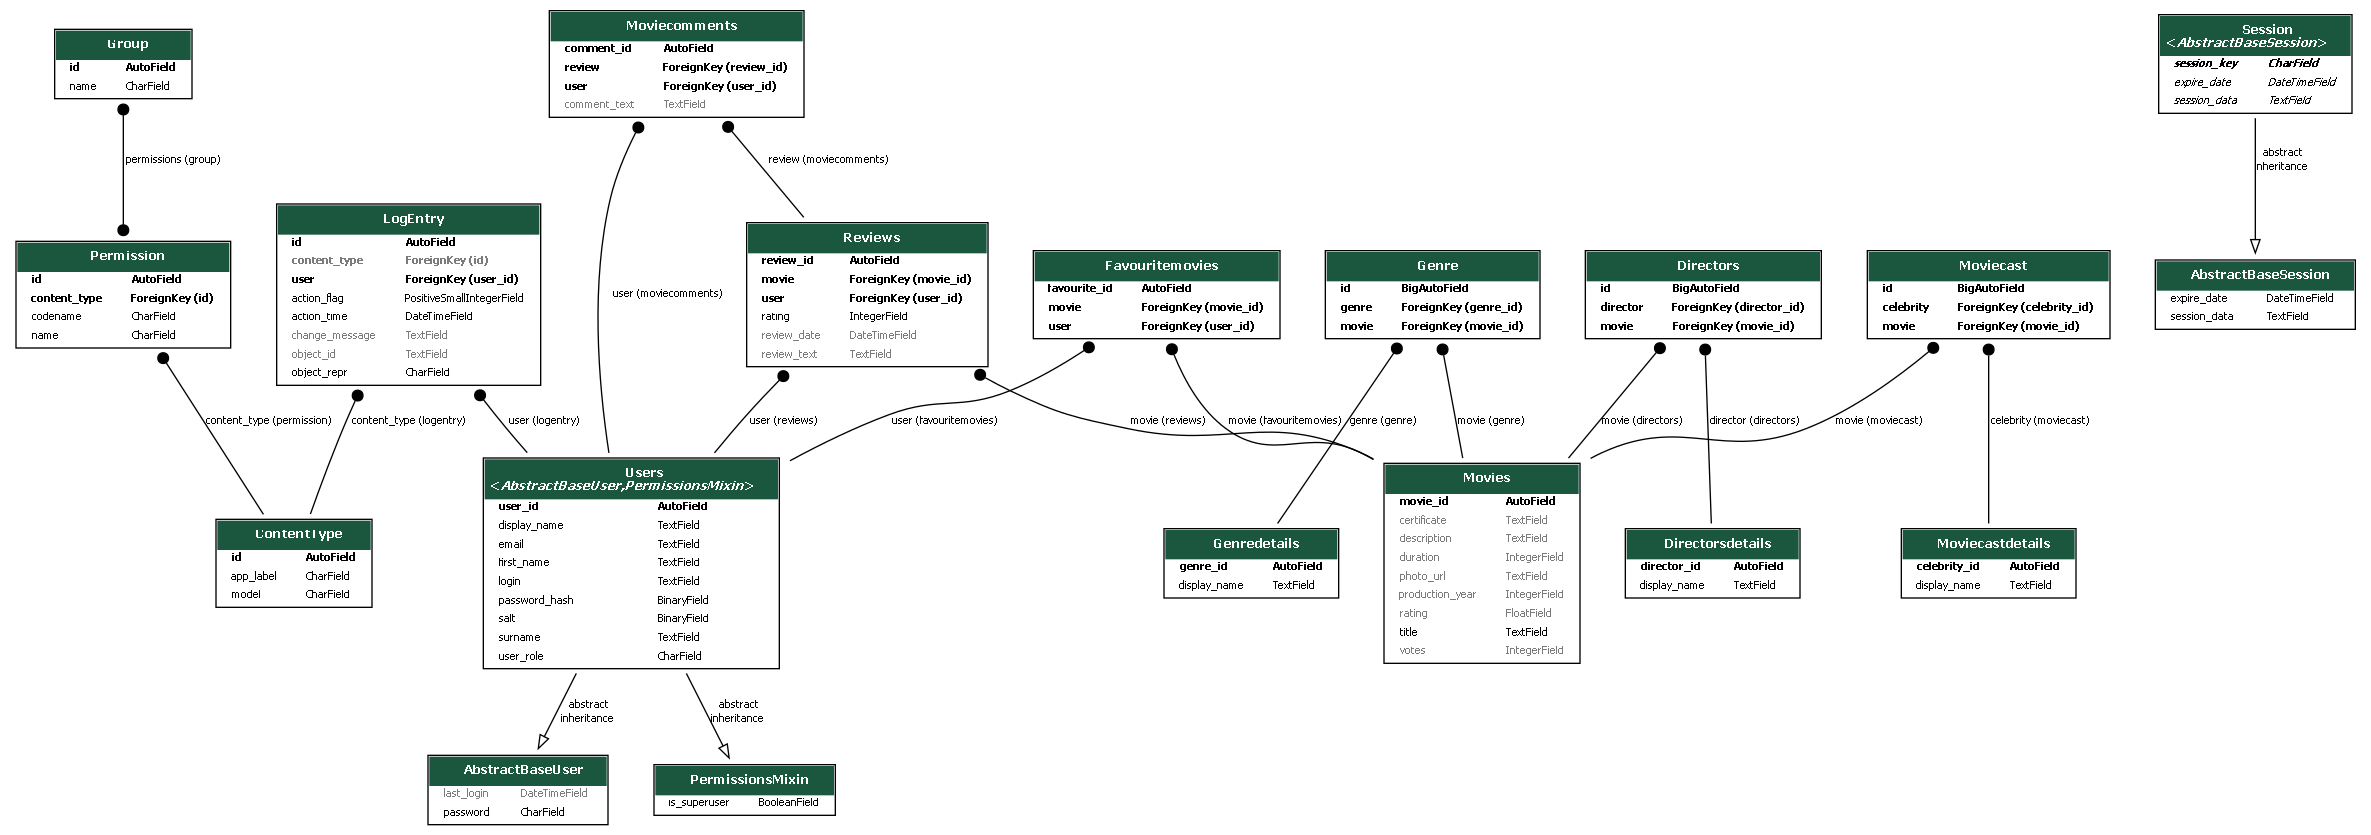
\includegraphics[width=0.95\textwidth]{backend/django_architecture.png}

	\caption{Diagram modelu relacyjnego w architekturze MVT}
	\label{fig:backend:model_diagram}
\end{figure}

\subsection{Podział na aplikacje Django}
Projekt jest podzielony na kilka aplikacji, z których każda obsługuje konkretne funkcjonalności:
\begin{itemize}
	\item \texttt{movie\_app}:
	      \begin{itemize}
		      \item Odpowiada za przeglądanie i wyszukiwanie filmów oraz generowanie rekomendacji filmowych dla użytkowników.
		      \item Definiuje modele filmów oraz logikę rekomendacyjną.
	      \end{itemize}
	\item \texttt{user\_app}:
	      \begin{itemize}
		      \item Zajmuje się rejestracją, logowaniem, zarządzaniem profilami użytkowników oraz autoryzacją.
		      \item Przechowuje dane użytkowników oraz zarządza sesjami.
	      \end{itemize}
	\item \texttt{review\_app}:
	      \begin{itemize}
		      \item Odpowiada za dodawanie recenzji do filmów oraz komentowanie recenzji innych użytkowników.
		      \item Zawiera modele recenzji i komentarzy oraz logikę zarządzającą tą funkcjonalnością.
	      \end{itemize}
	\item \texttt{recommendation\_app}:
	      \begin{itemize}
		      \item Odpowiada za tworzenie rekomendacji dla użytkowników
		      \item Zawiera model rekomendacji
	      \end{itemize}
\end{itemize}

\subsection{Baza danych}
Aplikacja korzysta z bazy danych PostgreSQL do przechowywania danych związanych z filmami, użytkownikami, recenzjami i komentarzami. Struktura bazy danych jest odzwierciedleniem modeli Django:
\begin{itemize}
	\item \textbf{Tabela filmów}: Zawiera dane o filmach (np. tytuł, reżyser, gatunek, ocena).
    \item \textbf{Tabela użytkowników}: Przechowuje dane o użytkownikach, w tym informacje o ich kontach i ustawieniach.
    \item \textbf{Tabela recenzji}: Przechowuje recenzje filmów napisane przez użytkowników.
    \item \textbf{Tabela komentarzy}: Przechowuje komentarze do recenzji filmów.
\end{itemize}

\subsection{Rekomendacje filmów}
Celem algorytmu rekomendacji jest dobranie zbioru filmów, które prawdopodobnie przypadną do gustu wskazanemu użytkownikowi. Algorytm ten polega na rekomendacjach wstawianych przez innych użytkowników oraz na ogólnej zależności gatunków filmów (jeśli użytkownikowi podoba się film kryminalny, to prawdopodobnie spodobają mu się inne filmy kryminalne).

Algorytm rekomendacji na początku pobiera ostatnio wystawione przez użytkownika pozytywne recenzje. Pozytywna recenzja jest definiowana jako recenzja, której ocena jest wyższa niż wskazany próg - próg ten wybrano na ocenę 4. Po pobraniu pozytywnych recenzji użytkownika, wywołany zostaje algorytm wyszukiwania filmów podobnych dla każdego pozytywnie ocenionego filmu.

Algorytm wyszukiwania podobnych filmów składa się z dwóch podalgorytmów. Pierwszy z nich, zwany \textit{rekomendacjami inteligentnymi}, sprawdza ostatnie pozytywne recenzje wybranego filmu. Następnie sprawdza on, jakie inne filmy zostały pozytywnie ocenione przez użytkowników, którzy te opinie wystawili, i zwraca odnalezione filmy. Druga część algorytmu, zwana \textit{rekomendacjami gatunkowymi}, sprawdza gatunki otrzymanego filmu i zwraca najpopularniejsze filmy z tych gatunków. Popularność filmu jest definiowana pod kątem oceny filmu, gdzie filmy o ocenie wyższej niż 4 są uznawane jako popularne. Otrzymane w ten sposób rekomendacje filmów są sortowane tak, aby najpierw pojawiły się filmy z algorytmu inteligentnego, a dopiero następnie pojawiały się filmy z rekomendacji gatunkowych.

\subsection{Warstwa komunikacji}
\begin{itemize}
	\item \textbf{Widoki Django (Views)}: Przetwarzają żądania HTTP, pobierają dane z modeli i generują odpowiedzi w postaci stron HTML. Widoki kontrolują logikę biznesową aplikacji, np. wyszukiwanie filmów, przetwarzanie recenzji czy rekomendacje.
    \item \textbf{Szablony (Templates)}: Szablony są odpowiedzialne za generowanie dynamicznych stron internetowych. Korzystają z języka szablonów Django, aby wyświetlać dane przekazywane przez widoki (np. listę filmów, recenzje, szczegóły użytkownika).
\end{itemize}

\subsection{Pliki konfiguracyjne}
Plik \texttt{settings.py} zawiera konfigurację całego projektu, w tym ustawienia bazy danych, konfigurację aplikacji, ustawienia statycznych plików, autoryzację oraz inne kluczowe ustawienia aplikacji.

\subsection{Statyczne zasoby i szablony}
\begin{itemize}
	\item \textbf{Pliki statyczne}: Zawierają zasoby takie jak CSS, JavaScript oraz obrazy, które są potrzebne do prawidłowego wyświetlania interfejsu użytkownika.
	\item \textbf{Szablony (HTML)}: Szablony HTML definiują, jak wyglądają strony internetowe generowane przez Django. Są zintegrowane z logiką w widokach i dynamicznie wyświetlają dane.
\end{itemize}

\subsection{API (Endpointy)}
\begin{itemize}
	\item \textbf{Główna aplikacja}
	\begin{itemize}
		\item \texttt{GET \slash }: Zwraca stronę główną aplikacji.
		\item \texttt{GET \slash about\slash }: Zwraca informację o aplikacji.
		\item \texttt{GET \slash admin\slash }: Zwraca stronę administratora.
	\end{itemize}
	\item \textbf{Filmy}
	\begin{itemize}
		\item \texttt{GET \slash movies\slash }: Zwraca listę wszystkich filmów.
		\item \texttt{GET \slash details\slash \{id\}\slash }: Zwraca szczegóły konkretnego filmu.
	\end{itemize}
	\item \textbf{Recenzje}
	\begin{itemize}
		\item \texttt{POST \slash reviews\slash add\_review\slash \{movie\_id\}\slash }: Dodaje nową recenzje dla filmu.
		\item \texttt{POST \slash reviews\slash add\_comment\slash \{review\_id\}\slash }: Dodaje komentarz do recenzji filmu.
	\end{itemize}
	\item \textbf{Użytkownicy}
	\begin{itemize}
		\item \texttt{GET \slash users\slash }: Zwraca listę wszystkich użytkowników.
		\item \texttt{GET \slash users\slash details\slash \{user\_id\}\slash }: Zwraca stronę użytkownika.
		\item \texttt{POST \slash users\slash login\slash }: Logowanie użytkownika.
		\item \texttt{POST \slash users\slash logout\slash }: Wylogowanie użytkownika.
		\item \texttt{POST \slash users\slash register\slash }: Rejestracja nowego użytkownika.
	\end{itemize}
\end{itemize}

\end{document}